\documentclass[letterpaper,12pt]{article}
\usepackage[utf8]{inputenc}
\usepackage[bottom]{footmisc}
\usepackage{graphicx}
\usepackage{amsmath}
\usepackage{amsthm}
\usepackage{amscd}
\usepackage{amssymb}
\usepackage{latexsym}
\usepackage{upref}
\usepackage[hidelinks]{hyperref}
\usepackage{cite}
\usepackage{subcaption}
\usepackage{xfrac}
\usepackage{bm}
\usepackage{mathtools}
\usepackage{ifthen}
\usepackage{optidef}
\usepackage{float}
\usepackage{dirtytalk}

\setlength{\textwidth}{6.4in}
\setlength{\textheight}{9.5in}
\setlength{\topmargin}{-1in}
\addtolength{\headheight}{0.0675in}
\setlength{\oddsidemargin}{0.2in}
\setlength{\evensidemargin}{0.2in}

\let\oldcite=\cite
\renewcommand\cite[1]{\ifthenelse{\equal{#1}{NEEDED}}{[citation~needed]}{\oldcite{#1}}}

\begin{document}

    \title{%
        1D Shallow-Water Wave Equation with Inferred Bathymetry\\
        \large A Physics-Informed Neural Network Approach
    }
    \author{%
        Nameika, Michael \\
        Thompson, Jonathan
    }
    \date{\today}
    \maketitle

    \begin{abstract}
        In this project, we examine a Physics-Informed Neural Network (PINN) approach to solving a 1D system of 
        shallow-water equations with variable bathymetry. We begin by stating the system of equations with variable
        bathymetry and from there derive the system of equations corresponding to a constant bathymetry with negligible
        frictional forces. From there, we solve the resulting system via pseudospectral methods for various boundary
        and initial conditions. We then use the results of this computation as sampled data with which to train a 
        Physics-Informed Neural Network (PINN); in this scheme, we treat the bathymetry as an unknown and allow the 
        neural network to infer the solution and bathymetry simultaneously. Lastly, we compare the results of the PINN
        approach to the results of the pseudospectral approach and discuss the advantages and disadvantages of each.
    \end{abstract}

    \section{Background}\label{sec:background}
        We first present the 1-D shallow-water equations for flood waves with variable bathymetry\cite{whitham1999_ch3}:

\begin{align*}
    h_t + (h v)_x &= 0 \\
    (h v)_t + \left[ hv^2 + \frac{1}{2} g h^2 \cos{(\alpha)} \right]_x &= g h \sin{(\alpha)} - C_f v^2
\end{align*}

where $v$ represents the average wave velocity, $h$ is the water depth, and $C_f$ is a friction
coefficient. Of these, $v$ and $h$ vary in time and space and while $C_f$ may, in general, vary with space we assume
it to be constant in this project. We expand the left-hand side of the second equation via the Chain Rule and 
substitute $h_t = -h_x v - h v_x$ from the first equation to find: 

\begin{align*}
    (h v)_t + \left[ hv^2 + \frac{1}{2} g h^2 \cos{(\alpha)} \right]_x 
        &= \left( h_t v + h v_t \right) + h_x v^2 + 2 h v v_x + \left[ \frac{1}{2} g h^2 \cos{(\alpha)} \right]_x \\
        &= -h_x v^2 - h v v_x + h v_t + h_x v^2 + 2 h v v_x + \left[ \frac{1}{2} g h^2 \cos{(\alpha)} \right]_x \\
        &=  h v v_x + h v_t + \left[ \frac{1}{2} g h^2 \cos{(\alpha)} \right]_x \\
        &=  h \left( v v_x + v_t + g h_x \cos{(\alpha)} + \frac{1}{2} g h [\cos{(\alpha)}]_x \right) \\
        &=  h \left( v v_x + v_t + g h_x \cos{(\alpha)} + g h [\cos{(\alpha)}]_x - \frac{1}{2} g h [\cos{(\alpha)}]_x \right) \\
        &=  h \left( v_t + \left[ \frac{v^2}{2} + g h \cos{(\alpha)} \right]_x - \frac{1}{2} g h [\cos{(\alpha)}]_x \right).
\end{align*}

\pagebreak
We may express our system in conservation form as

$$
    \textbf{u}_t + \left[ F(\textbf{u}) \right]_x = S(\textbf{u})
$$

where (after dividing through by $h$)

$$
\textbf{u} = \begin{pmatrix}
    h \\
    v
\end{pmatrix}, \quad F(\textbf{u}) = \begin{pmatrix}
    hv \\
    \frac{v^2}{2} + g h \cos{(\alpha)}
\end{pmatrix}, \quad S(\textbf{u}) = \begin{pmatrix}
    0 \\
    g \sin{(\alpha)} - C_f \frac{v^2}{h} + \frac{1}{2} g h [\cos{(\alpha)}]_x
\end{pmatrix}.
$$

We expand $[F(\textbf{u})]_x$ to find:

$$
[F(\textbf{u})]_x = \begin{pmatrix}
    h v_x + h_x v \\
    v v_x + g h_x \cos{(\alpha)} + g h [\cos{(\alpha)}]_x
\end{pmatrix} = \begin{pmatrix}
    v                & h \\
    g \cos{(\alpha)} & v
\end{pmatrix} \begin{pmatrix}
    h \\
    v
\end{pmatrix}_x + \begin{pmatrix}
    0 \\
    g h [\cos{(\alpha)}]_x
\end{pmatrix}
$$

and so our system becomes

$$
\textbf{u}_t + A(\textbf{u}) \textbf{u}_x = \tilde{S}(\textbf{u})
$$

where 

$$
A = \begin{pmatrix}
    v                & h \\
    g \cos{(\alpha)} & v
\end{pmatrix}, \quad \tilde{S} = \begin{pmatrix}
    0 \\
    g h \sin{(\alpha)} (1 - \alpha_x) - C_f \frac{v^2}{h}
\end{pmatrix}.
$$


    \section{Methodology}\label{sec:proposed-methodology}

    \subsection{Pseudospectral Methods}\label{subsec:pseudospectral-methodology}
        To simulate experimental observations and generate a reference solution, we adopt the approach used by Fabien \cite{fabien2014spectral} and utilize a Fourier collocation method along 
with fourth-order Runge-Kutta time stepping. Recall the definition of the Fourier Transform of a differentiable function 
$f$:

$$
\mathcal{F}(f(x)) \equiv \int_{-\infty}^{\infty}f(x)e^{-ikx}dx
$$

where $\hat{f}(k) \equiv \mathcal{F}(f(x))$ is a function in $k$. From this, we also have the inverse Fourier transform:

$$
f(x) = \frac{1}{2\pi}\int_{-\infty}^{\infty} \hat{f}(k)e^{ikx}dk
$$

\noindent Differentiating both sides of the above equation with respect to $k$ yields

$$
\frac{df}{dx} = ik\frac{1}{2\pi}\int_{-\infty}^{\infty}\hat{f}(x)e^{ikx}dx
$$

\noindent and so

$$
\hat{f'}(k) = ik\hat{f}(k).
$$

Taking the inverse Fourier transform of the above equation yields the general form for the derivative of a function with 
respect to its Fourier transform:

$$
f'(x) = \mathcal{F}^{-1}(ik\mathcal{F}(f(x))).
$$

\noindent Extending this to the $n^{th}$ derivative yields:

$$
f^{(n)}(x) = \mathcal{F}^{-1}((ik)^n\mathcal{F}(f(x))).
$$

We apply these results to the SWE system with periodic boundary conditions, which takes the following form:

\begin{align*}
    \begin{bmatrix}
        h\\
        uh
    \end{bmatrix}_t
    + 
    \begin{bmatrix}
        uh\\
        hu^2 + \frac{gh^2}{2}
    \end{bmatrix}_x
    =
    \begin{bmatrix}
        0\\
        -ghB_x
    \end{bmatrix}
\end{align*}    

To compute the spatial derivative, we differentiate in the Fourier domain and apply the inverse Fourier transform 
$\mathcal{F}^{-1}$ to the resulting expression. Upon doing so, our system becomes

\begin{align*}
    \begin{bmatrix}
        h\\
        uh
    \end{bmatrix}_t
    + 
    \mathcal{F}^{-1}\left(ik\mathcal{F}\left(\begin{bmatrix}
        uh\\
        hu^2 + \frac{gh^2}{2}
    \end{bmatrix} \right)\right)
    = 
    \begin{bmatrix}
        0\\
        -ghB_x
    \end{bmatrix}.
\end{align*}

We approximate the time derivative with a fourth-order Runge-Kutta time-stepping scheme. This system is expressed in 
terms of the time derivatives of $u$ and $uh$; we therefore rewrite the second equation in the system in 
terms of $u$ and $uh$ to find:

$$
\renewcommand*{\arraystretch}{1.5}
\begin{bmatrix}
    h\\
    uh
\end{bmatrix}_t = -\begin{bmatrix}
    \mathcal{F}^{-1}(ik\mathcal{F}(uh))\\
    ghB_x + \mathcal{F}^{-1}(ik\mathcal{F}((uh)^2/h + gh^2/2)) 
\end{bmatrix} = \begin{bmatrix}
    F_1(u,uh)\\
    F_2(u,uh)
\end{bmatrix}.
$$

\noindent Given $h$ at step $n$, our update step to compute $h_{n+1}$ is

\begin{align*}
    k_{1,h} &= dt\frac{L}{2\pi}F_1(h_n, uh_n)\\
    k_{2,h} &= dt\frac{L}{2\pi}F_1(h_n + k_{1,h}/2, uh_n)\\
    k_{3,h} &= dt\frac{L}{2\pi}F_1(h_n + k_{2,h}/2, uh_n)\\
    k_{4,h} &= dt\frac{L}{2\pi}F_1(h_n + k_{3,h}, uh_n)\\
    h_{n+1} &= h_n + \frac{1}{6}(k_{1,h} + 2k_{2,h} + 2k_{3,h} + k_{4,h})
\end{align*}

\noindent As for the quantity $uh$, our update $(uh)_{n+1}$ is given by

\begin{align*}
    k_{1,uh} &= dt\frac{L}{2\pi}F_2(h_{n+1}, uh_n)\\
    k_{2,uh} &= dt\frac{L}{2\pi}F_2(h_{n+1}, uh_n + k_{1,uh}/2)\\
    k_{3,uh} &= dt\frac{L}{2\pi}F_2(h_{n+1}, uh_n + k_{2,uh}/2)\\
    k_{4,uh} &= dt\frac{L}{2\pi}F_2(h_{n+1}, uh_n + k_{3,uh})\\
    uh_{n+1} &= \frac{1}{6}(k_{1,uh} + 2k_{2,uh} + 2k_{3,uh} + k_{4,uh})
\end{align*}

where $dt$ is the time step and $\frac{L}{2\pi}$ the domain scaling factor. To simulate our desired experimental 
measurement data, we solve the SWE system subject to various (sinusoidal) initial conditions and bathymetry functions. 
In the homogeneous scheme, we impose a bathymetry function that is identically zero; for the inhomogeneous system, we
impose a sinusoidal bathymetry. The exact functions used for these computations are described in Section 
\ref{sec:results} and results of these computations for the homogenous system are shown in Figures 
\ref{fig:homogeneous_pseudospectral_swe_height} and \ref{fig:homogeneous_pseudospectral_swe_velocity}; inhomogeneous 
results are shown in Figure \ref{fig:inhomogeneous_pseudospectral_swe_velocity}.

    \subsection{Physics-Informed Neural Networks}\label{subsec:pinn-methodology}
        In the Physics-Informed Neural Network approach, we build upon the methodology developed by Raissi et. al. 
\cite{raissi_physics-informed_2019} and approximate the solution to a system of partial differential equations with a
neural network. In particular, we seek neural network solution surrogates to (possibly nonlinear) equations of the form 

$$
u_t + \mathcal{N}[u; \lambda] = 0, \quad x \in \Omega, \quad t \in [0, T]
$$

where $\mathcal{N}$ is a parameterized spatial differentiation operator and $\Omega$ is a subset of $\mathbb{R}^n$. In 
the case of the shallow water equations, we have:

$$
\mathcal{N}[u; \lambda] = [F(u; \lambda)]_x - S(u; \lambda), \quad u = \begin{bmatrix}
    h \\
    v \\
    \alpha
\end{bmatrix}, \quad \text{and} \quad \lambda = C_f.
$$

We approximate the solution to the PDE by a neural network $U(x, t; \theta)$, where $\theta$ represents the parameters
of the neural network which is trained by minimizing the PDE residual. We define the residual 
$f \coloneqq u_t + \mathcal{N}[u]$ and, for given collocation points $\{x_i, t_i\}$, define the (mean-squared) loss 
function for the neural network in terms of $f$:

$$
MSE_f = \frac{1}{N_f} \sum_{i=1}^{N_f} |f(x_i, t_i)|^2
$$

Furthermore, when sampled data for the solution is available, we enforce consistency of the neural network with respect 
to measured data by introducing a second loss function for the sampled data:

$$
MSE_u = \frac{1}{N_u} \sum_{i=1}^{N_u} |U(x_i, t_i; \theta) - u(x_i, t_i)|^2
$$

where $u(x_i, t_i)$ represents a particular data sample and $U(x_i, t_i; \theta)$ the neural network prediction at that
sample point. We may therefore view the process of finding a neural network that satisfies the PDE as the unconstrained 
optimization problem:

\begin{mini*}
    {\theta}{MSE_f + MSE_u}{}{}
\end{mini*}

For this project, we generate an artificial data set for the $MSE_u$ term by first solving the PDE via pseudospectral 
methods and sampling the numerical solution at various temporospatial points. We train the neural network using DeepXDE
\cite{lu_deepxde_2021}, a Python library based on Tensorflow and PyTorch for solving PDEs via PINNs. 
            
    \subsection{Optimization Algorithms}
        \subsubsection{L-BFGS}
            
The limited memory BFGS algorithm (L-BFGS) approximates the inverse Hessian (denoted by $H$) using $m$ past updates of 
the position and the gradient at the position. These updates are used to implicitly approximate the inverse Hessian. In 
contrast to the BFGS algorithm, BFGS approximates the Hessian matrix, as opposed to the inverse Hessian.


In a manner similar to the BFGS algorithm, we define

\begin{align*}
    s_k &= x_{k+1} - x_k\\
    y_k &= \nabla f(x_{k+1}) - \nabla f(x_k).
\end{align*}

We also define $\rho = \frac{1}{y_k^Ts_k}$. The update for the inverse Hessian is given as

$$
    H_{k+1} = (I - \rho_ks_ky_k^T)H_k(I - \rho_ky_ks_k^T) + \rho_ks_ks_k^T
$$

For the low-storage aspect, we define a sequence of vectors $q_{k-m}, \dots, q_k$ at a fixed $k$ to be 
$q_k = \nabla f(x_k)$ and $q_i = (I - \rho_iy_is_i^T)q_{i+1}$. Define another sequence of vectors $z_{k-m},\dots, z_k$ 
as $z_i = H_iq_i$. The value of $z_k$ is said to be an ascent direction. The L-BFGS algorithm is given in Figure 
\ref{fig:L-BFGS-Algorithm},

\pagebreak

\begin{figure}[h]
    \centering
    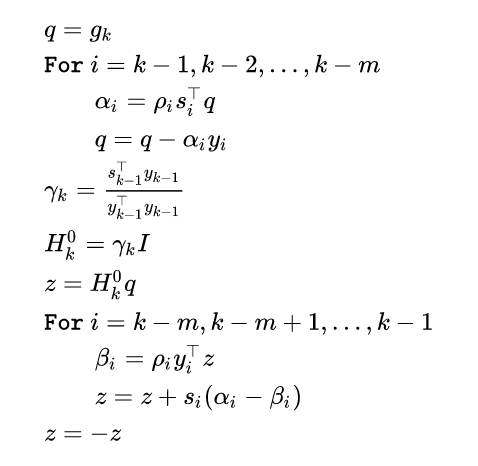
\includegraphics[width=0.5\textwidth]{images/L-BFGS-Algorithm.png}
    \caption{Outline of the L-BFGS algorithm. Taken from Wikipedia.}
    \label{fig:L-BFGS-Algorithm}
\end{figure}

where $g_k = \nabla f(x_k)$. This gives a search direction for the minimization problem.
        \subsubsection{Adam}
            Stochastic Gradient Descent (SGD) is also employed for the machine learning process. SGD is an iterative method that is a stochastic approximation of typical gradient descent. SGD tends to achieve faster computation time of iterations at the expense of a slower convergence rate. In typical gradient descent, the gradient of the objective function is computed over the entire domain  of data points, whereas SGD takes sampled subsets of the domain and approximates the gradient over this random sample. That is, in typical gradient descent for machine learning, our problem may look like
\begin{align*}
    \text{minimize} \hspace{1em} f(x) = \frac{1}{2}\sum_{i \in D} \|N(x) - y_i \|^2\\
\end{align*}
Where $N(x)$ is the neural network approximation and $y_i$ is the measured data. The associated update step is given by
\[x_{k+1} = x_k - \alpha \nabla f(x)\]
With SGD, we restrict our attention to $i \in S \subset D$ so that the update step looks like
\[x_{k+1} = x_k - \alpha \nabla f_i(x)\]
where $\nabla f_i(x)$ is the estimated gradient of $f$ over a domain sample.
\newline\newline


A variation of SGD that was utilized was the Adam SGD method. Adam (Adaptive Moment Estimation) runs averages with exponential \say{forgetting} of both gradients and second moments of gradients. Given parameters $w^{(t)}$ and a loss function $L^{(t)}$ with $t$ indexing the current training iteration starting from 0, the Adam parameter update is given by
\begin{figure}[H]
    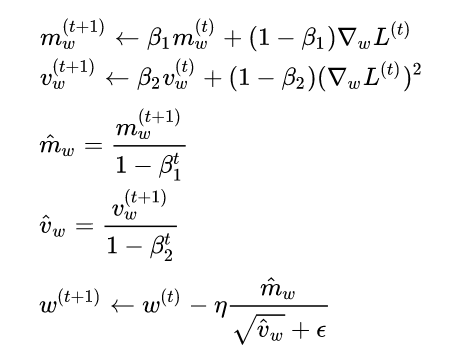
\includegraphics[scale = 1]{images/adam.png}
    \centering
    \caption{Outline of the Adams stochastic gradient descent algorithm. Taken from Wikipedia.}
\end{figure}
with $\epsilon$ small (i.e. $10^{-8})$ and $\beta_1$ (i.e. 0.9) and $\beta_2$ (i.e. 0.999) are called the forgetting factors for the gradients and second moments of the gradients. The square root and squaring operations are done elementwise. 

    \section{Comparison}\label{sec:comparison}
    
    \section{Conclusions and Future Work}\label{sec:conclusion}

    \pagebreak

    \bibliographystyle{plain}
    \bibliography{refs}

    \pagebreak
    \appendix

\end{document}
